Spočtěte určitý integrál
\begin{enumerate}

	\item $\int_{-1}^1 |x| \dx$,

		\solution{
			Absolutní hodnota se nedá pěkně integrovat, tak si integrál rozdělíme na dva následující větou:
			pro libovolná $a < b < c \in \mathbb{R}$ platí následující rovnost (pokud obě strany dávají smysl)
			$$\int_a^c f(x) \dx = \int_a^b f(x) \dx + \int_b^c f(x) \dx$$

			Použití je následovné:
			absolutní hodnota je spojitá funkce, tedy daný integrál existuje, obdobně $\pm x$:
			$$\int_{-1}^1 |x| \dx = \int_{-1}^0 (-x) \dx + \int_0^1 x \dx = - \int_{-1}^0 x\dx + \int_0^1 x \dx = $$
			$$= -\left[\frac{x^2}{2}\right]_{-1}^0 + \left[\frac{x^2}{2}\right]_0^1 = -(0-1/2)+(1/2-0)=1$$

			Geometrický význam vidíme na Obrázku~\ref{fig:abs}.
			\begin{figure}[H]
				\centering
				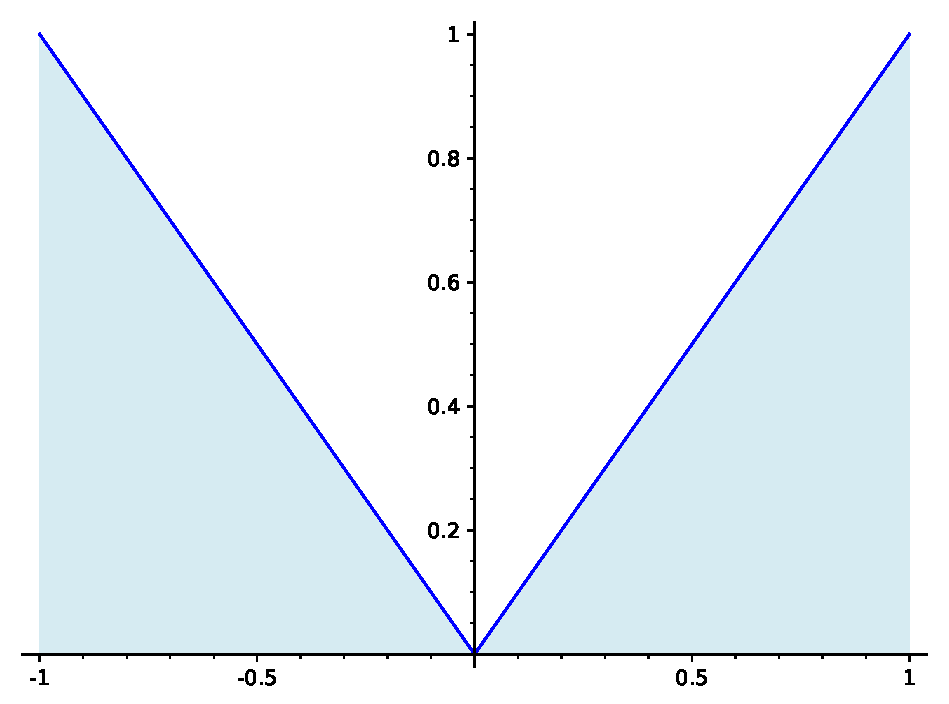
\includegraphics{cviceni_13/fig/abs.pdf}
				\caption{$\int_{-1}^1 |x| \dx = 1$}
				\label{fig:abs}
			\end{figure}
		}

	\item $\int_{1/e}^e |\ln x| \dx$,

		\solution{
			Primitivní funkce k funkci $\ln(x)$ (bez absolutní hodnoty) je 
			$$\int \ln x \dx = x (\ln x -1) +C$$
			pak
			$$\int_{1/e}^e |\ln x| \dx = -\int_{1/e}^1 \ln x \dx + \int_1^e \ln x \dx = 
			 -\left[x (\ln x -1)\right]_{1/e}^1 + \left[x (\ln x -1)\right]_1^e =$$
			$$= -(1(0-1)-\frac{1}{e}(-1-1)) + (e(1-1)-1(0-1)) = -(-1+\frac{2}{e})+(0+1) = 2-\frac{2}{e}$$

			Geometrický význam vidíme na Obrázku~\ref{fig:lnx}.
			\begin{figure}[H]
				\centering
				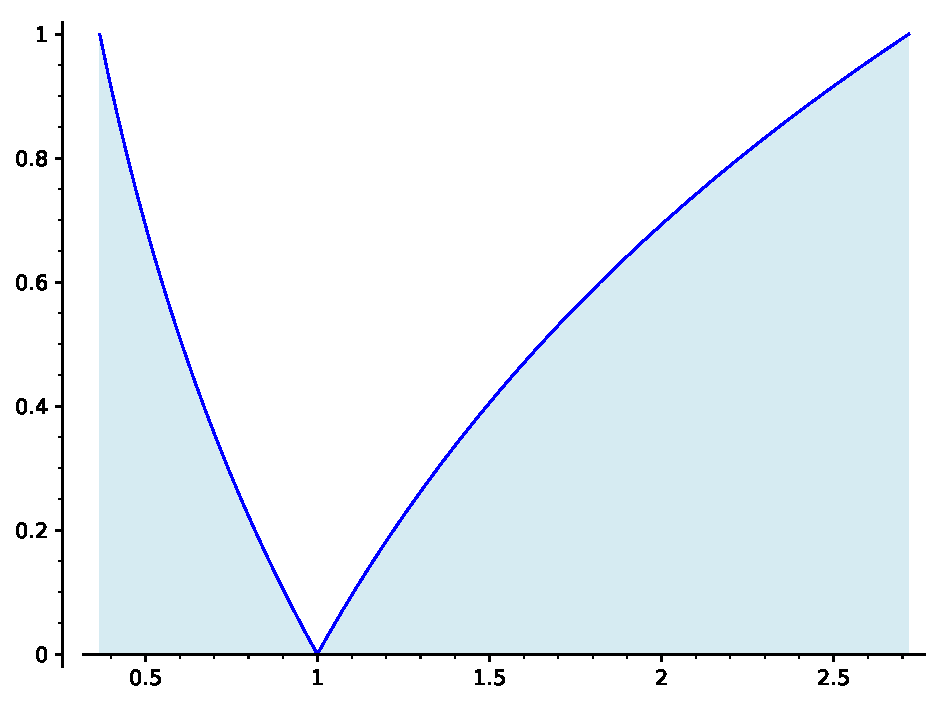
\includegraphics{cviceni_13/fig/lnx.pdf}
				\caption{$\int_{1/e}^e |\ln x| \dx = 2 - \frac{2}{e}$}
				\label{fig:lnx}
			\end{figure}
		}

\end{enumerate}

